\documentclass[11pt]{article}
\usepackage[T1]{fontenc}
\usepackage[utf8]{inputenc}
\usepackage{lmodern,microtype}
\usepackage[margin=1in]{geometry}
\usepackage{amsmath,amssymb,mathtools,bm}
\usepackage{graphicx,booktabs,tabularx,array}
\usepackage{xcolor,enumitem,caption,float}
\usepackage[section]{placeins}
\usepackage{tikz}
\usetikzlibrary{arrows.meta,positioning,fit}
\usepackage[numbers,sort&compress]{natbib}
\usepackage{xurl}
\usepackage{hyperref}
\usepackage[nameinlink,noabbrev]{cleveref}

\hypersetup{colorlinks=true,linkcolor=blue!45!black,
  citecolor=green!35!black,urlcolor=blue!55!black,
  pdftitle={Learning an Agent-Centered Geometry of Quantum Possibility}}
\captionsetup{font=small,labelfont=bf}
\setlist{nosep,leftmargin=1.6em}
\setlength{\emergencystretch}{2em}
\newcommand{\E}{\mathbb E}
\newcommand{\Prob}{\mathbb P}
\newcommand{\R}{\mathbb R}
\newcommand{\Tr}{\operatorname{Tr}}
\newcommand{\softmax}{\operatorname{softmax}}
\newcommand{\JS}{D_{\mathrm{JS}}}
\newcommand{\doi}[1]{\href{https://doi.org/#1}{doi:#1}}

\title{\textbf{Learning an Agent-Centered Geometry of Quantum Possibility}\\
\large Predictive State, Goal-Conditioned Control, and Directed Reachability
from Measurement Experience Alone}
\author{RL Experiments Project\\
\small Author information omitted for review}
\date{August 2026}

\begin{document}
\maketitle

\begin{abstract}
We study a deliberately austere quantum-control problem. An artificial agent
may choose a measurement and observe its classical outcome, but it is never
given the quantum state, Kraus operators, Born probabilities, Hamiltonian, or
tomographic estimates. Its experience is only a sequence of interventions and
consequences. The scientific objective is therefore broader than quantum
control: what operational representation of an unknown world can be learned
from first-person experience, and can many possible aims be organized into a
useful geometry?

We compare finite-history tabular Q-learning, goal-conditioned recurrent
Q-learning, and a predictive multi-goal gated recurrent unit (GRU). The full
agent jointly learns reward value, one-step outcome prediction, a
stochastic-shortest-path cost, and goal embeddings regularized by policy
similarity. Five environment families vary Hilbert-space dimension, hidden
initial state, measurement strength, informational completeness, and outcome
alphabet, including a qubit symmetric informationally complete (SIC)
measurement and mutually unbiased qutrit bases. Thirty-six agents are trained
across six scenarios, three backends, and two seeds.

The predictive geometry agent has the best macro-average success (80.5\%),
versus 79.1\% for finite-history Q-learning and 77.7\% for the reward-only GRU,
but no backend dominates every environment and neural seed variance is large.
Euclidean goal-embedding distance correlates moderately with held-out policy
distance (mean Spearman $\rho=0.54$) and more weakly with independent
trajectory distance ($\rho=0.31$). Learned reachability is directionally
informative but not metrically calibrated: blank-history cost correlates
$r=0.47$ with empirical conditional hitting time and has mean absolute error
1.75 interventions. Intervention maps nevertheless reveal a legible directed
structure in which outcomes reduce distance to matching goals while often
increasing distance to alternatives. Goal geometry is thus a productive
diagnostic and planning language, but its metric interpretation requires
stronger validation.
\end{abstract}

\noindent\textbf{Keywords:} reinforcement learning; quantum measurement;
partial observability; predictive state; goal-conditioned control;
reachability; representation learning; QBism

\tableofcontents
\newpage

\section{Introduction}

Quantum control is usually described from the standpoint of an external
modeler, who writes down a state $\rho$, a Hamiltonian, and control or
measurement operators before optimizing a protocol. Model-free quantum control
instead asks what can be learned through interaction, an approach already used
for quantum feedback, state preparation, and error correction
\cite{fosel2018,sivak2022,borah2021}.

This work imposes a stricter informational boundary. The agent chooses an
intervention $a_t$ and receives a classical outcome $o_t$. It is not given
$\rho_t$, measurement operators, expectation values, fidelities, or
tomography. Its information at time $t$ is
\begin{equation}
 h_t=(a_1,o_1,\ldots,a_{t-1},o_{t-1}). \label{eq:history}
\end{equation}
This interface is compatible with QBism's emphasis on an agent's actions,
experiences, and expectations \cite{fuchs2014}, although the algorithms do not
assume or establish any interpretation of quantum theory. Agent-centered here
describes the information boundary.

The central difficulty is partial observability. An external physicist may use
$\rho_t$ as a Markov state, but the learner cannot. It needs an internal
summary $z_t=F(h_t)$ retaining distinctions relevant to prediction and control.
This motivates three objects that must remain distinct:
\begin{enumerate}
 \item \textbf{predictive state}: which histories imply the same future
 intervention/outcome statistics;
 \item \textbf{strategic goal geometry}: which goals call for similar policies
 or trajectories;
 \item \textbf{directed reachability}: how difficult a goal is from the
 agent's present history.
\end{enumerate}
Our methodological contribution is a validation framework comparing learned
Euclidean goal embeddings with held-out policy behavior, trajectory
signatures, empirical hitting times, finite-horizon success curves, and
intervention-induced changes in all goal distances.

\begin{figure}[t]
\centering
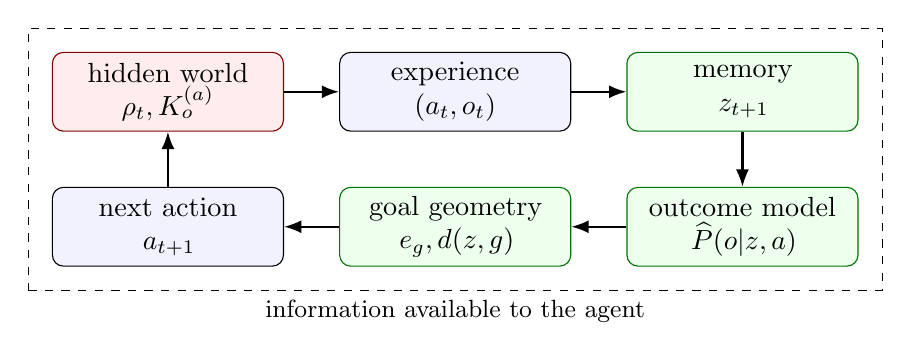
\begin{tikzpicture}[
 box/.style={draw,rounded corners,align=center,minimum height=10mm,
 text width=27mm,fill=blue!5},
 hidden/.style={box,fill=red!7,draw=red!50!black},
 learned/.style={box,fill=green!7,draw=green!45!black},
 arrow/.style={-{Latex[length=2.2mm]},thick},node distance=7mm and 7mm]
\node[hidden] (world) {hidden world\\$\rho_t,K_o^{(a)}$};
\node[box,right=of world] (exp) {experience\\$(a_t,o_t)$};
\node[learned,right=of exp] (state) {memory\\$z_{t+1}$};
\node[learned,below=of state] (model) {outcome model\\$\widehat P(o|z,a)$};
\node[learned,left=of model] (geo) {goal geometry\\$e_g,d(z,g)$};
\node[box,left=of geo] (action) {next action\\$a_{t+1}$};
\draw[arrow] (world)--(exp); \draw[arrow] (exp)--(state);
\draw[arrow] (state)--(model); \draw[arrow] (model)--(geo);
\draw[arrow] (geo)--(action); \draw[arrow] (action)--(world);
\node[draw,dashed,fit=(exp)(state)(model)(geo)(action),inner sep=3mm,
 label=below:{\small information available to the agent}] {};
\end{tikzpicture}
\caption{The operational learning loop. Quantum variables in red are private
to the simulator. The agent constructs state, prediction, and goal-relative
reachability from experienced action/outcome pairs.}
\label{fig:loop}
\end{figure}

\section{Hidden quantum dynamics}
\label{sec:quantum}

\subsection{Quantum instruments and backaction}

A finite-dimensional quantum state is externally represented by a positive
semidefinite unit-trace density operator $\rho$. A measurement action $a$ has a
Kraus operator $K_o^{(a)}$ for each classical outcome $o$, with physical
completeness \cite{kraus1983,nielsen2010}
\begin{equation}
 \sum_o K_o^{(a)\dagger}K_o^{(a)}=I. \label{eq:complete}
\end{equation}
The hidden simulator samples and updates by
\begin{align}
 p(o|\rho,a)&=\Tr(K_o^{(a)}\rho K_o^{(a)\dagger}), \label{eq:born}\\
 \rho'&=\frac{K_o^{(a)}\rho K_o^{(a)\dagger}}{p(o|\rho,a)}. \label{eq:update}
\end{align}
Measurement therefore both supplies information and changes the conditions
governing future experiences. This backaction is why reachability is naturally
directed. The learner never evaluates \cref{eq:born,eq:update}; it receives only
the sampled integer outcome.

For a projective basis $\{|b_o\rangle\}$, one may take
$K_o=|b_o\rangle\langle b_o|$. The qubit worlds use Pauli $Z$, $X$, and $Y$
bases. Their noncommutativity creates incompatible preparation strategies.
The unsharp binary instruments use axis projectors $P_+,P_-$ and strength
$q\in(1/2,1)$:
\begin{align}
 K_0&=\sqrt q\,P_+ +\sqrt{1-q}\,P_-,&
 K_1&=\sqrt{1-q}\,P_+ +\sqrt q\,P_- . \label{eq:weak}
\end{align}
At $q=0.5$ the outcome is uninformative; as $q\to1$ the operation approaches a
projective measurement. We use $q=0.8$.

A SIC-POVM in dimension $d$ contains $d^2$ equiangular rank-one effects and is
informationally complete \cite{renes2004}. For the qubit tetrahedral SIC,
\begin{equation}
 E_i=\frac{I+\bm r_i\cdot\bm\sigma}{4},\qquad \sum_{i=0}^3E_i=I,
\end{equation}
where $\bm r_i$ are tetrahedral Bloch vectors; we use the positive square-root
instrument $K_i=\sqrt{E_i}$. This tests mixed outcome alphabets: projective
actions have two outcomes while the SIC has four. Invalid logits are masked.

Two bases $\{|e_j\rangle\}$ and $\{|f_k\rangle\}$ are mutually unbiased when
$|\langle e_j|f_k\rangle|^2=1/d$ for all $j,k$. Certainty in one becomes a
uniform distribution in the other. MUBs formalize complementarity and support
tomography \cite{durt2010}. The qutrit world uses three projective MUBs.

\subsection{Environment catalog}

\begin{table}[t]
\centering
\caption{World/state scenarios. The hidden state is reset each episode.}
\label{tab:envs}
\begin{tabularx}{\textwidth}{@{}lclXc@{}}
\toprule
Environment & $d$ & Initial state & Measurement actions & Goals\\
\midrule
qubit-zx-weak & 2 & $|1\rangle$ & projective $Z,X$; weak $Z$ & 7\\
qubit-zx-weak & 2 & $|+\rangle$ & projective $Z,X$; weak $Z$ & 7\\
qubit-pauli & 2 & $|+i\rangle$ & projective $Z,X,Y$ & 7\\
qubit-unsharp & 2 & $I/2$ & weak $Z,X,Y$ & 6\\
qubit-pauli-sic & 2 & $I/2$ & projective $Z,X,Y$; tetrahedral SIC & 9\\
qutrit-mub & 3 & $|2\rangle$ & three projective MUBs & 8\\
\bottomrule
\end{tabularx}
\end{table}

Operational state is relative to the available interventions. With an
informationally incomplete repertoire, physically different density operators
may imply identical statistics for everything an agent can do. Adding a SIC
action or moving from qubit to qutrit may require a richer predictive
representation. This motivates varying worlds rather than only random seeds.

\section{Reinforcement learning from first principles}
\label{sec:rl}

\subsection{MDPs, return, and value}

Reinforcement learning concerns sequential decisions with delayed consequences
\cite{sutton2018}. A finite Markov decision process is
$(\mathcal S,\mathcal A,P,R,\gamma)$: states, actions, a transition/reward law,
and discount $\gamma\in[0,1]$. The Markov property says the present state
contains all past information needed to predict the next transition. A policy
$\pi(a|s)$ is a distribution over actions. The discounted return is
\begin{equation}
 G_t=R_{t+1}+\gamma R_{t+2}+\gamma^2R_{t+3}+\cdots.
\end{equation}
The action value is $Q^\pi(s,a)=\E_\pi[G_t|S_t=s,A_t=a]$. Optimal value obeys
the Bellman equation
\begin{equation}
 Q^*(s,a)=\E[R_{t+1}+\gamma\max_{a'}Q^*(S_{t+1},a')|s,a]. \label{eq:bellman}
\end{equation}
The value of acting now is immediate reward plus the best discounted value
available afterward.

\subsection{Q-learning and exploration}

Q-learning estimates \cref{eq:bellman} without knowing $P$ or $R$
\cite{watkins1992}. From transition $(s_t,a_t,r_t,s_{t+1})$, it forms target
$y_t=r_t+\gamma\max_{a'}Q(s_{t+1},a')$ (or $r_t$ at termination) and updates
\begin{equation}
 Q(s_t,a_t)\leftarrow Q(s_t,a_t)+\alpha[y_t-Q(s_t,a_t)]. \label{eq:qlearn}
\end{equation}
The bracket is the temporal-difference error. Q-learning is off-policy: the
target assumes a greedy continuation even when behavior explores. With
$\epsilon$-greedy behavior, a uniformly random action is chosen with
probability $\epsilon$ and a maximizing action otherwise. Classical convergence
guarantees require finite tabular state/action spaces, suitable learning rates,
and sufficient visitation \cite{watkins1992}; they do not automatically extend
to nonlinear recurrent networks.

\subsection{Partial observability and predictive state}

Here the simulator's $\rho_t$ could be Markov, but is hidden. The problem is a
POMDP \cite{kaelbling1998}; the policy is $\pi(a_t|h_t)$, not
$\pi(a_t|\rho_t)$. The tabular baseline truncates experience to
\begin{equation}
 s_t^{(L)}=(g,j_t,(a_{t-L},o_{t-L}),\ldots,(a_{t-1},o_{t-1})), \label{eq:tabstate}
\end{equation}
where $g$ is the goal and $j_t$ its progress. This is transparent, but $L$ is
arbitrary, its state count grows exponentially, and similar histories share no
strength unless identical.

Predictive-state representations instead characterize state by
action-conditional predictions \cite{littman2001}. Ideally,
\begin{equation}
 h\sim_{\rm pred}h'\Longleftrightarrow
 \Prob(o_{1:k}|a_{1:k},h)=\Prob(o_{1:k}|a_{1:k},h')
\end{equation}
for every future test. Our recurrent vector is only an approximation, trained
for control and one-step prediction. The predictive-state view supplies the
interpretation and a future validation standard.

\subsection{GRU memory and deep temporal-difference learning}

A recurrent network maintains fixed-size memory
\begin{equation}
 z_{t+1}=F_\theta(z_t,a_t,o_t). \label{eq:memory}
\end{equation}
With $x_t$ the concatenated action/outcome embedding, a GRU
\cite{cho2014} can be written
\begin{align}
 r_t&=\sigma(W_rx_t+U_rz_t+b_r),&
 u_t&=\sigma(W_ux_t+U_uz_t+b_u),\\
 \widetilde z_{t+1}&=\tanh(W_hx_t+U_h(r_t\odot z_t)+b_h),&
 z_{t+1}&=(1-u_t)\odot\widetilde z_{t+1}+u_t\odot z_t.
\end{align}
Reset and update gates learn what to forget and retain. Complete episodes are
replayed through the GRU so late losses can alter earlier encoding:
backpropagation through time. A slowly moving target network stabilizes TD
targets, following deep Q-learning practice \cite{mnih2015}:
\begin{equation}
 \theta^-\leftarrow(1-\tau)\theta^-+\tau\theta. \label{eq:target}
\end{equation}

\subsection{Evaluation principles}

RL evaluation is difficult because training changes the data distribution and
results vary across seeds. Reproducibility studies warn that few-run point
estimates can reverse rankings \cite{henderson2018,agarwal2021}. Evaluation
should separate exploratory training from held-out greedy behavior, show
per-task and aggregate results, and distinguish success probability from speed.
Conditional duration can reward a reckless policy because failures are
excluded. We therefore treat success as primary, label conditional steps, and
retain full finite-horizon success curves. With two seeds, this study is
exploratory rather than inferential.

\section{Sequence goals and three geometries}
\label{sec:geometry}

\subsection{Goal-conditioned control}

A goal is an ordered sequence
$g=((a_1^g,o_1^g),\ldots,(a_m^g,o_m^g))$. Other events may occur between
checkpoints. Progress $j_t$ is allowed because it is computed from the
experienced history. Rewards are 10 for completion, 1 for an intermediate
checkpoint, and $-0.01$ otherwise. A goal-conditioned value
$Q(z,g,j,a)$ lets the same remembered history support different policies.

\subsection{Symmetric strategic similarity}

Each known goal has embedding $e_g\in\R^k$. Distance
$D_E(g,h)=\|e_g-e_h\|_2$ is intended to mean similarity of strategy, not labels.
At encountered state $z$, define
\begin{equation}
 \pi_g(a|z,j)=\softmax_a(Q(z,g,j,a)/T). \label{eq:policy}
\end{equation}
For policies $p,q$, Jensen--Shannon divergence is
\begin{equation}
 \JS(p,q)=\tfrac12D_{\rm KL}(p\|m)+\tfrac12D_{\rm KL}(q\|m),
 \quad m=\tfrac12(p+q).
\end{equation}
Its square root is a metric \cite{endres2003}. The regularizer is
\begin{equation}
 \mathcal L_{\rm geom}=\frac1{|\mathcal P|}\sum_{g<h}
 [\|e_g-e_h\|_2-c\sqrt{\JS(\pi_g,\pi_h)}]^2. \label{eq:geoloss}
\end{equation}
The policy target is detached. Geometry is therefore partly imposed. Held-out
agreement tests generalization; it is not spontaneous emergence without bias.

\subsection{Trajectory similarity}

Local policy similarity may miss long-horizon differences. From held-out
rollouts we build
\begin{equation}
 \phi(g)=[\text{action frequencies},\text{ action/outcome frequencies},
 \text{ normalized duration},\text{ success rate}]
\end{equation}
and $D_{\rm traj}(g,h)=\|\phi(g)-\phi(h)\|_2$. This resembles successor
features, which describe policies by expected future features and support
transfer \cite{barreto2017}, although our signature is diagnostic rather than a
learned successor model.

\subsection{Directed reachability and displacement}

Let $\tau_g$ be first completion time. The ideal intervention-count distance is
\begin{equation}
 d^*(z,g,j)=\min_\pi\E_\pi[\tau_g|z,j]. \label{eq:hitting}
\end{equation}
This is a stochastic shortest-path problem \cite{bertsekas1991} with Bellman
form
\begin{equation}
 d^*(z,g,j)=1+\min_a\sum_oP(o|z,a)
 d^*(F(z,a,o),g,j'(a,o)). \label{eq:costbellman}
\end{equation}
The network learns positive action cost $C(z,g,j,a)$ and sets
$d(z,g,j)=\min_a C(z,g,j,a)$. Its target is 1 on completion and otherwise
\begin{equation}
 y_t^C=1+\min_{a'}C_{\theta^-}(z_{t+1},g,j_{t+1},a'). \label{eq:costtarget}
\end{equation}
This is directed: measurement can destroy conditions needed to return.

For $N$ goals, the agent's goal-relative position is
\begin{equation}
 \bm D(z)=(d(z,g_1),\ldots,d(z,g_N)).
\end{equation}
An observed intervention produces displacement
$\Delta\bm D_t=\bm D(z_{t+1})-\bm D(z_t)$. Negative coordinates mean closer,
positive farther. With the learned predictor, a contemplated action has
\begin{equation}
 \E[d'_g|z,a]=\sum_o\widehat P(o|z,a)d(F(z,a,o),g), \label{eq:planning}
\end{equation}
which provides a route to model-based planning.

A scalar mean hides risk, so we also estimate
\begin{equation}
 R_g(z,T)=\Prob(\tau_g\le T|z,\pi_g). \label{eq:curve}
\end{equation}
This parallels distributional RL's emphasis on distributions rather than only
expected return \cite{bellemare2017}.

\section{Architecture and experimental protocol}
\label{sec:methods}

All agents share one interaction protocol and receive only goal ID, progress,
action, outcome, reward, and termination. The \textbf{tabular} state is
\cref{eq:tabstate} with $L=4$. The \textbf{GRU} concatenates memory, a learned
goal embedding, and one-hot progress before an MLP Q-head. The
\textbf{predictive geometry GRU} adds a goal-independent outcome head,
goal-conditioned cost head, and \cref{eq:geoloss}. Its prediction loss is
\begin{equation}
 \mathcal L_{\rm pred}=-\log\widehat P_\theta(o_t|z_t,a_t),
\end{equation}
computed before incorporating $o_t$. The full loss is
\begin{equation}
 \mathcal L=\mathcal L_Q+\lambda_P\mathcal L_{\rm pred}
 +\lambda_C\mathcal L_C+\lambda_G\mathcal L_{\rm geom}. \label{eq:loss}
\end{equation}

\begin{figure}[t]
\centering
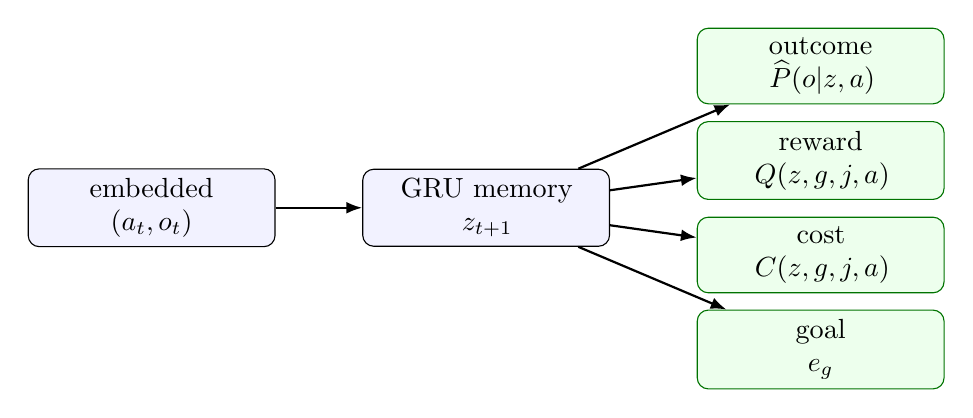
\begin{tikzpicture}[
 box/.style={draw,rounded corners,align=center,minimum height=9mm,
 text width=29mm,fill=blue!5},
 head/.style={box,fill=green!7,draw=green!45!black},
 arrow/.style={-{Latex[length=2mm]},thick},node distance=7mm and 11mm]
\node[box] (pair) {embedded\\$(a_t,o_t)$};
\node[box,right=of pair] (gru) {GRU memory\\$z_{t+1}$};
\node[head,right=of gru,yshift=18mm] (pred) {outcome\\$\widehat P(o|z,a)$};
\node[head,right=of gru,yshift=6mm] (q) {reward\\$Q(z,g,j,a)$};
\node[head,right=of gru,yshift=-6mm] (cost) {cost\\$C(z,g,j,a)$};
\node[head,right=of gru,yshift=-18mm] (emb) {goal\\$e_g$};
\draw[arrow] (pair)--(gru); \draw[arrow] (gru)--(pred);
\draw[arrow] (gru)--(q); \draw[arrow] (gru)--(cost);
\draw[arrow] (gru)--(emb);
\end{tikzpicture}
\caption{Shared recurrent representation and four learning objectives. Outcome
prediction is goal-independent; reward and cost are goal-conditioned.}
\label{fig:network}
\end{figure}

Goals are sampled uniformly. Each episode resets hidden state, memory, and
progress. Trajectories are replayed once for backpropagation through time;
reward and cost use \cref{eq:target}; gradients are clipped to norm 5.

\begin{table}[t]
\centering
\caption{Production configuration.}
\label{tab:hypers}
\begin{tabular}{@{}ll@{\qquad}ll@{}}
\toprule
Training episodes/run & 400 & Evaluation episodes/goal & 100\\
Geometry episodes/goal & 40 & Horizon & 15\\
Discount $\gamma$ & 0.95 & Tabular $\alpha$ & 0.10\\
History length & 4 & Neural learning rate & $10^{-3}$\\
$\epsilon$ start/end/decay & $1/.05/.99$ & Target $\tau$ & .02\\
GRU/goal dimensions & 32/6 & Interaction embedding & 8\\
$\lambda_P,\lambda_C,\lambda_G$ & $.5,.5,.05$ & Geometry scale & 2\\
Weak strength & .8 & Seeds & 0,1\\
\bottomrule
\end{tabular}
\end{table}

Evaluation disables exploration. Separate geometry rollouts evaluate every
goal-conditioned policy at each state, build trajectory signatures, compare
blank-history cost to hitting time, estimate \cref{eq:curve}, and group
displacements by action/outcome. PCA is used only to visualize embeddings; all
distance comparisons use original dimensions.

The study contains 14,400 training episodes (107,804 interventions), 26,400
evaluation episodes (179,342 interventions), and 3,520 geometry episodes. An
exact manifest, tidy CSVs, model weights, and plots are saved. Eighteen tests
verify quantum validity, outcome masks, reproducibility, goals, runner
semantics, every agent, and geometry utilities.

\section{Results}
\label{sec:results}

\subsection{Control performance}

\begin{figure}[p]
\centering
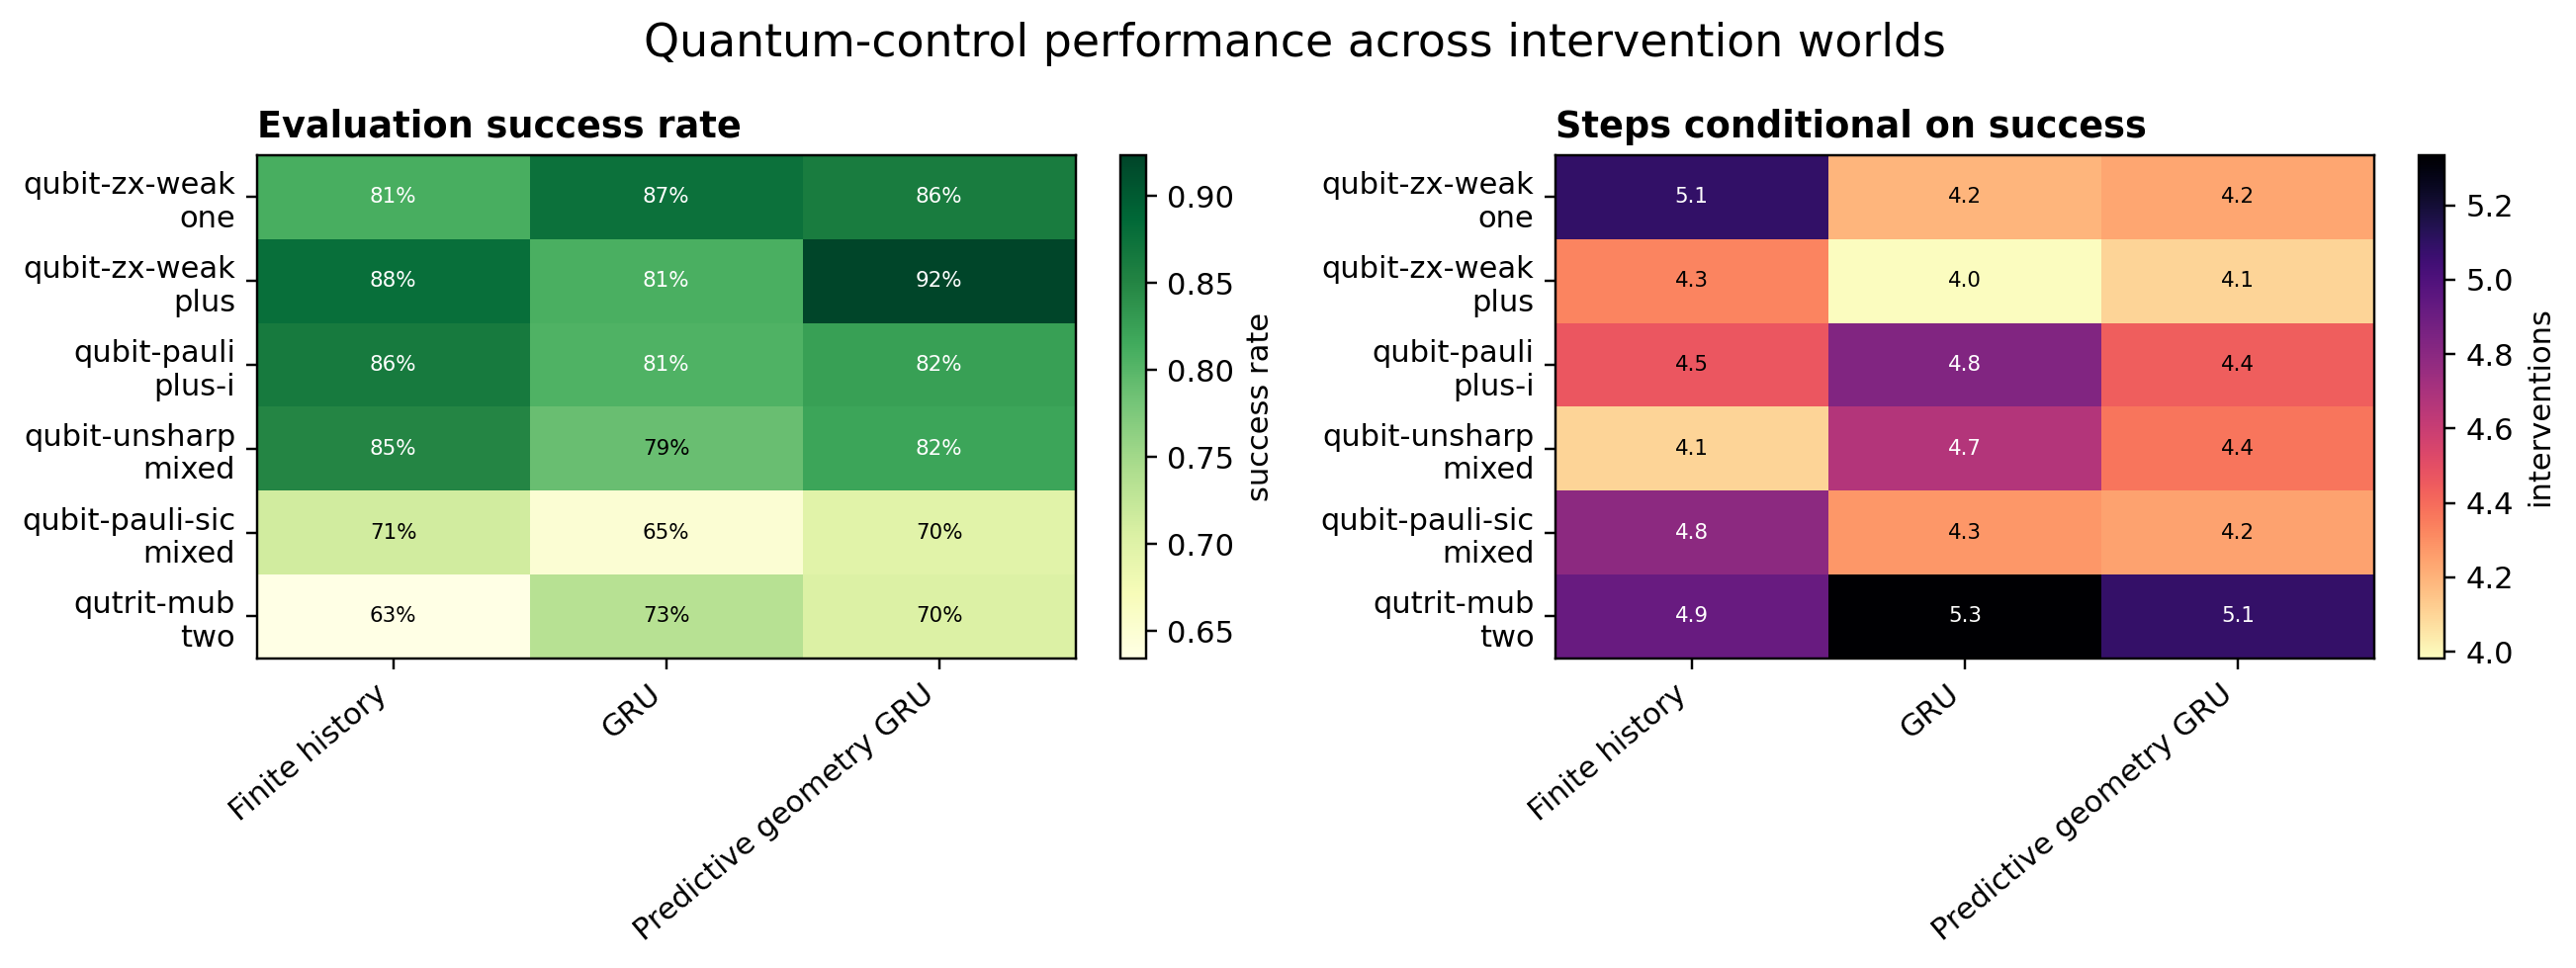
\includegraphics[width=\textwidth]{results/comparative/plots/performance_comparison.png}
\caption{Held-out success and conditional intervention count, averaged over two
seeds. Conditional steps exclude failures and must be read beside success.}
\label{fig:performance}
\end{figure}

\begin{table}[t]
\centering
\caption{Success rate, mean $\pm$ sample standard deviation over two seeds.
Bold is the largest scenario mean.}
\label{tab:success}
\small
\begin{tabularx}{\textwidth}{@{}Xccc@{}}
\toprule
World / state & Finite history & GRU & Predictive geometry GRU\\
\midrule
Z/X/weak-Z / $|1\rangle$ & $.810\pm.012$ & $\bm{.874\pm.038}$ & $.861\pm.035$\\
Z/X/weak-Z / $|+\rangle$ & $.878\pm.009$ & $.809\pm.063$ & $\bm{.924\pm.005}$\\
Pauli / $|+i\rangle$ & $\bm{.863\pm.018}$ & $.806\pm.057$ & $.825\pm.169$\\
unsharp / $I/2$ & $\bm{.849\pm.008}$ & $.788\pm.080$ & $.820\pm.071$\\
Pauli+SIC / $I/2$ & $\bm{.713\pm.006}$ & $.649\pm.027$ & $.697\pm.172$\\
qutrit MUB / $|2\rangle$ & $.634\pm.034$ & $\bm{.734\pm.082}$ & $.703\pm.015$\\
\midrule
Macro-average & $.791$ & $.777$ & $\bm{.805}$\\
\bottomrule
\end{tabularx}
\end{table}

No backend dominates. Recurrent memory helps on the qutrit and original
$|1\rangle$ scenarios; tabular learning leads on Pauli, unsharp, and Pauli+SIC;
the full model is strongest from $|+\rangle$. Macro conditional steps are 4.62
(tabular), 4.55 (GRU), and 4.41 (full), but success remains primary.

Neural instability is substantial. Mean absolute seed gaps are 2.1 percentage
points for tabular, 8.2 for GRU, and 11.0 for the full model; the largest full
gap is 24.3. Both recurrent agents have zero success on the three-checkpoint
qutrit goal, while tabular reaches 15\%. The plain GRU also has zero success on
the two-step $Z0\_SIC0$ goal.

\begin{figure}[p]
\centering
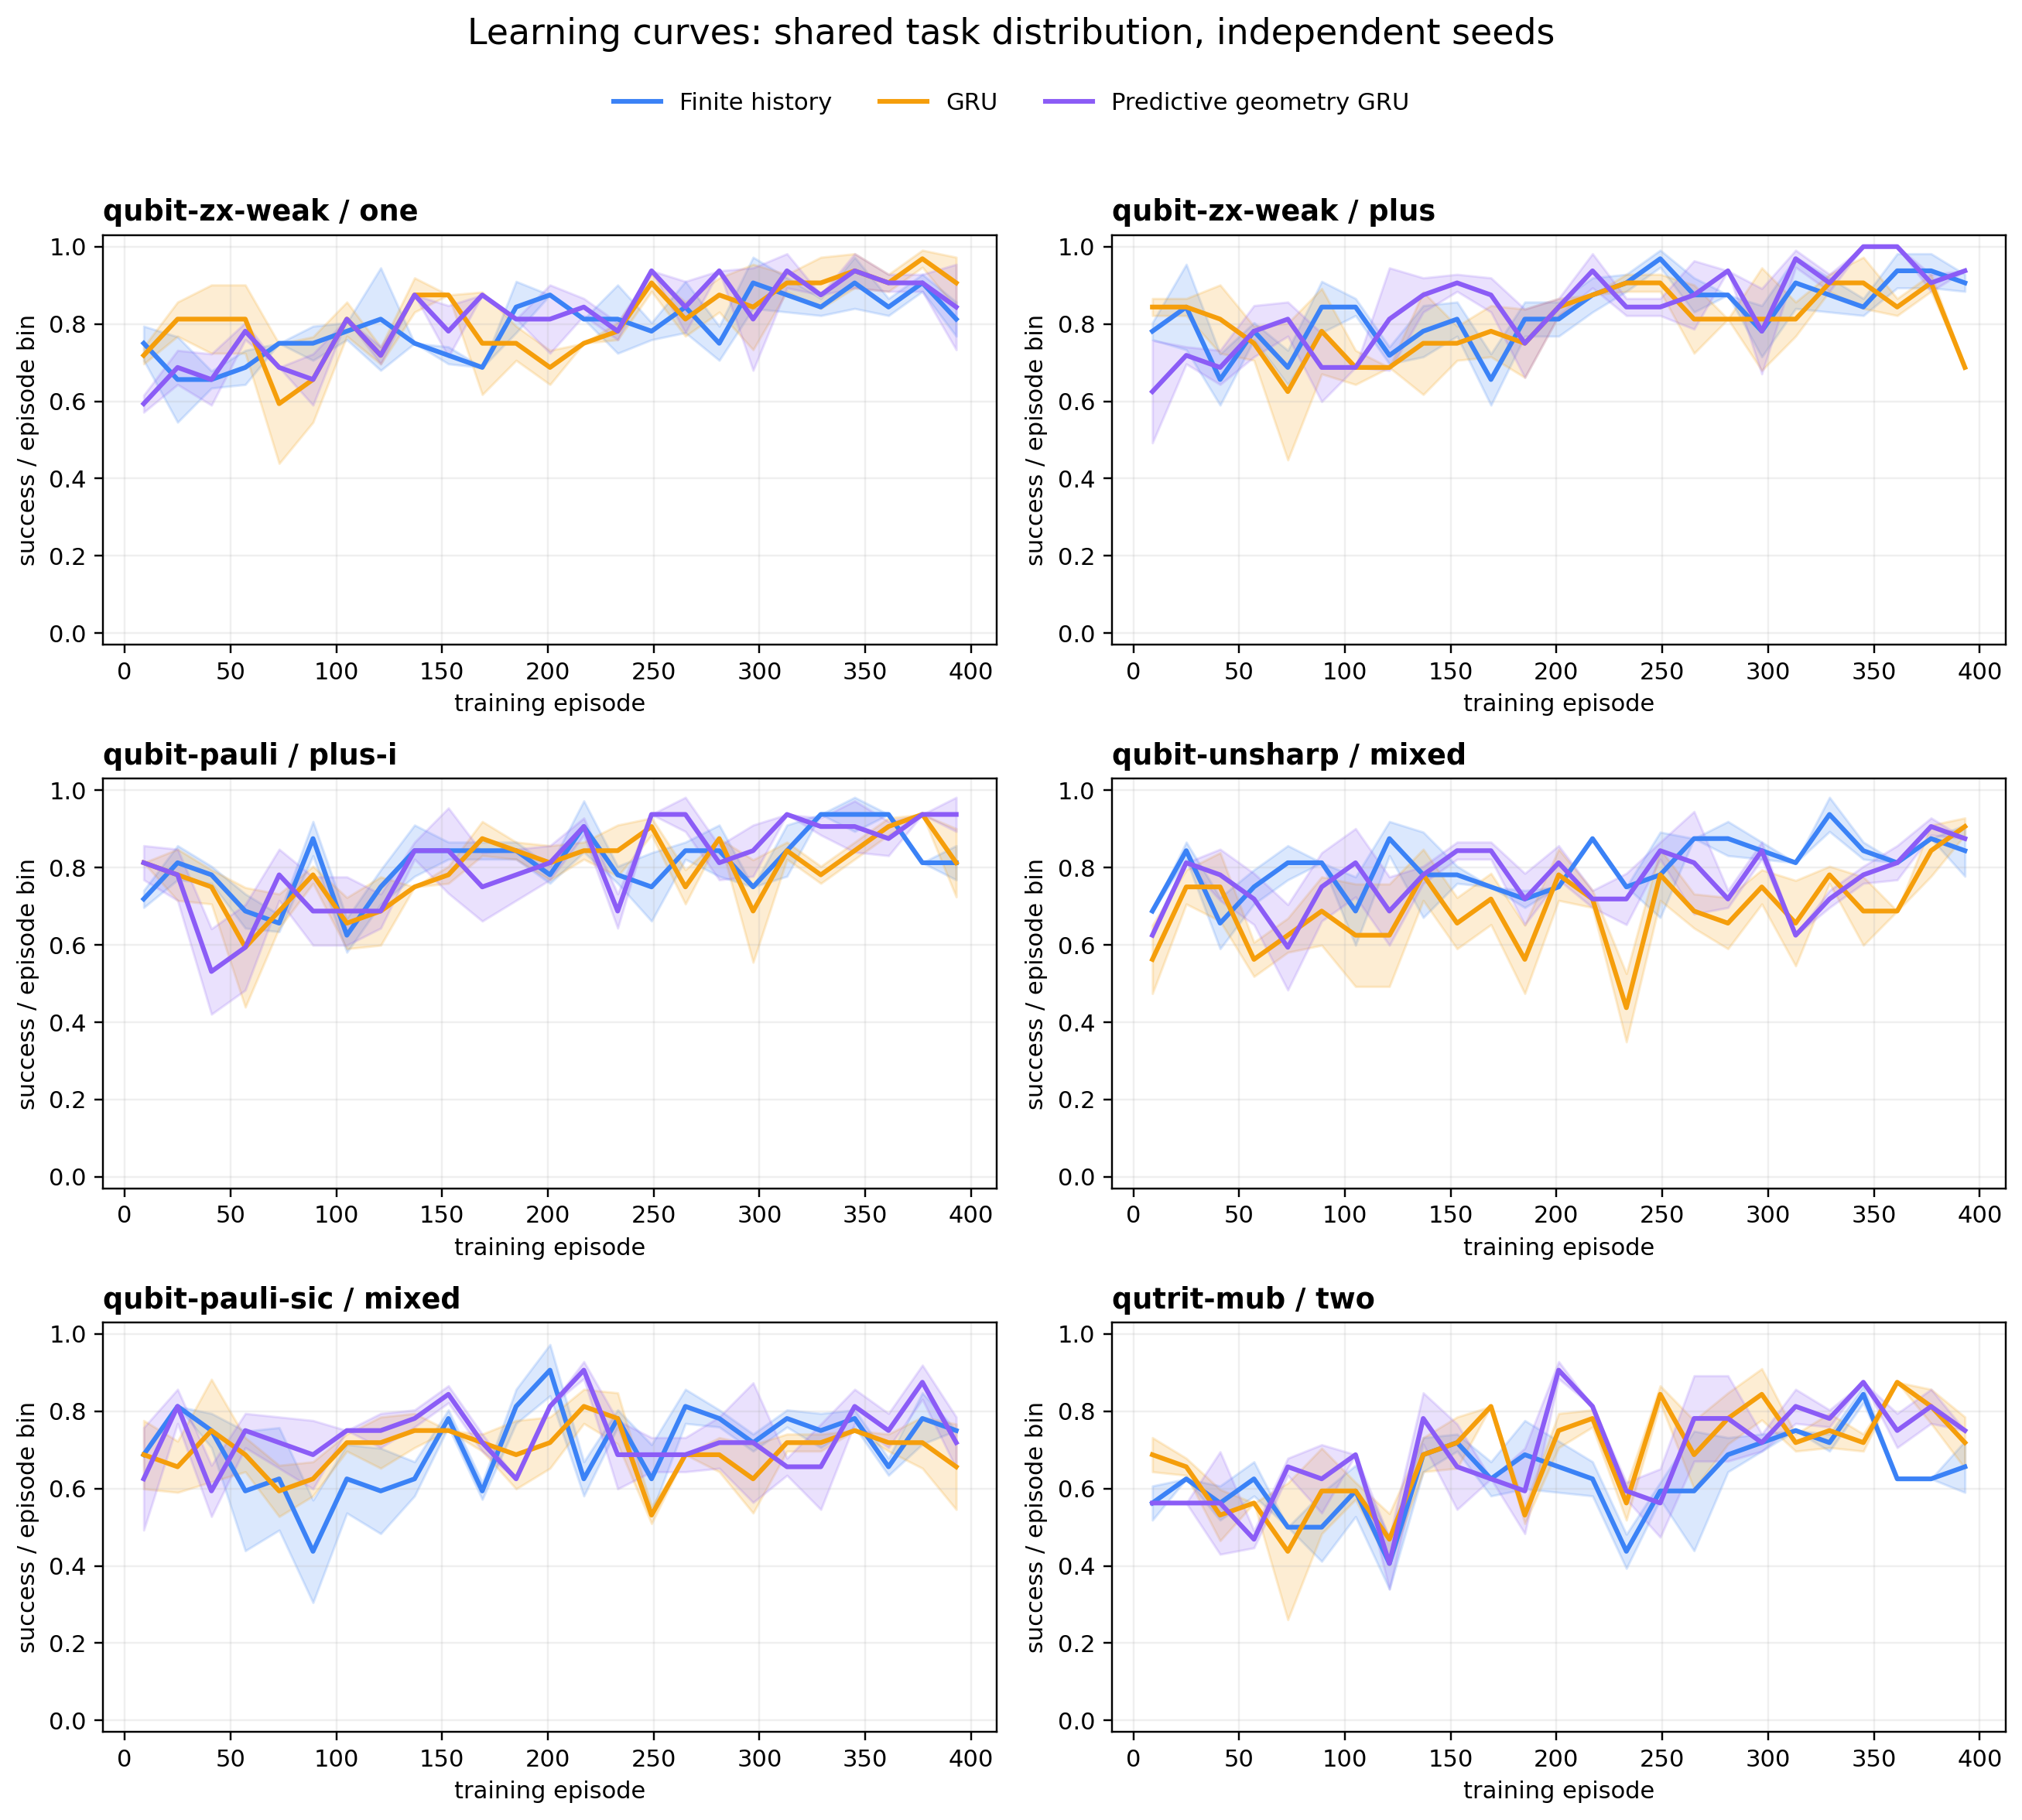
\includegraphics[width=.93\textwidth]{results/comparative/plots/learning_curves.png}
\caption{Binned exploratory training success. Shading is standard error over
only two seeds and is descriptive, not a reliable interval.}
\label{fig:learning}
\end{figure}

\subsection{Goal-geometry validation}

\begin{figure}[p]
\centering
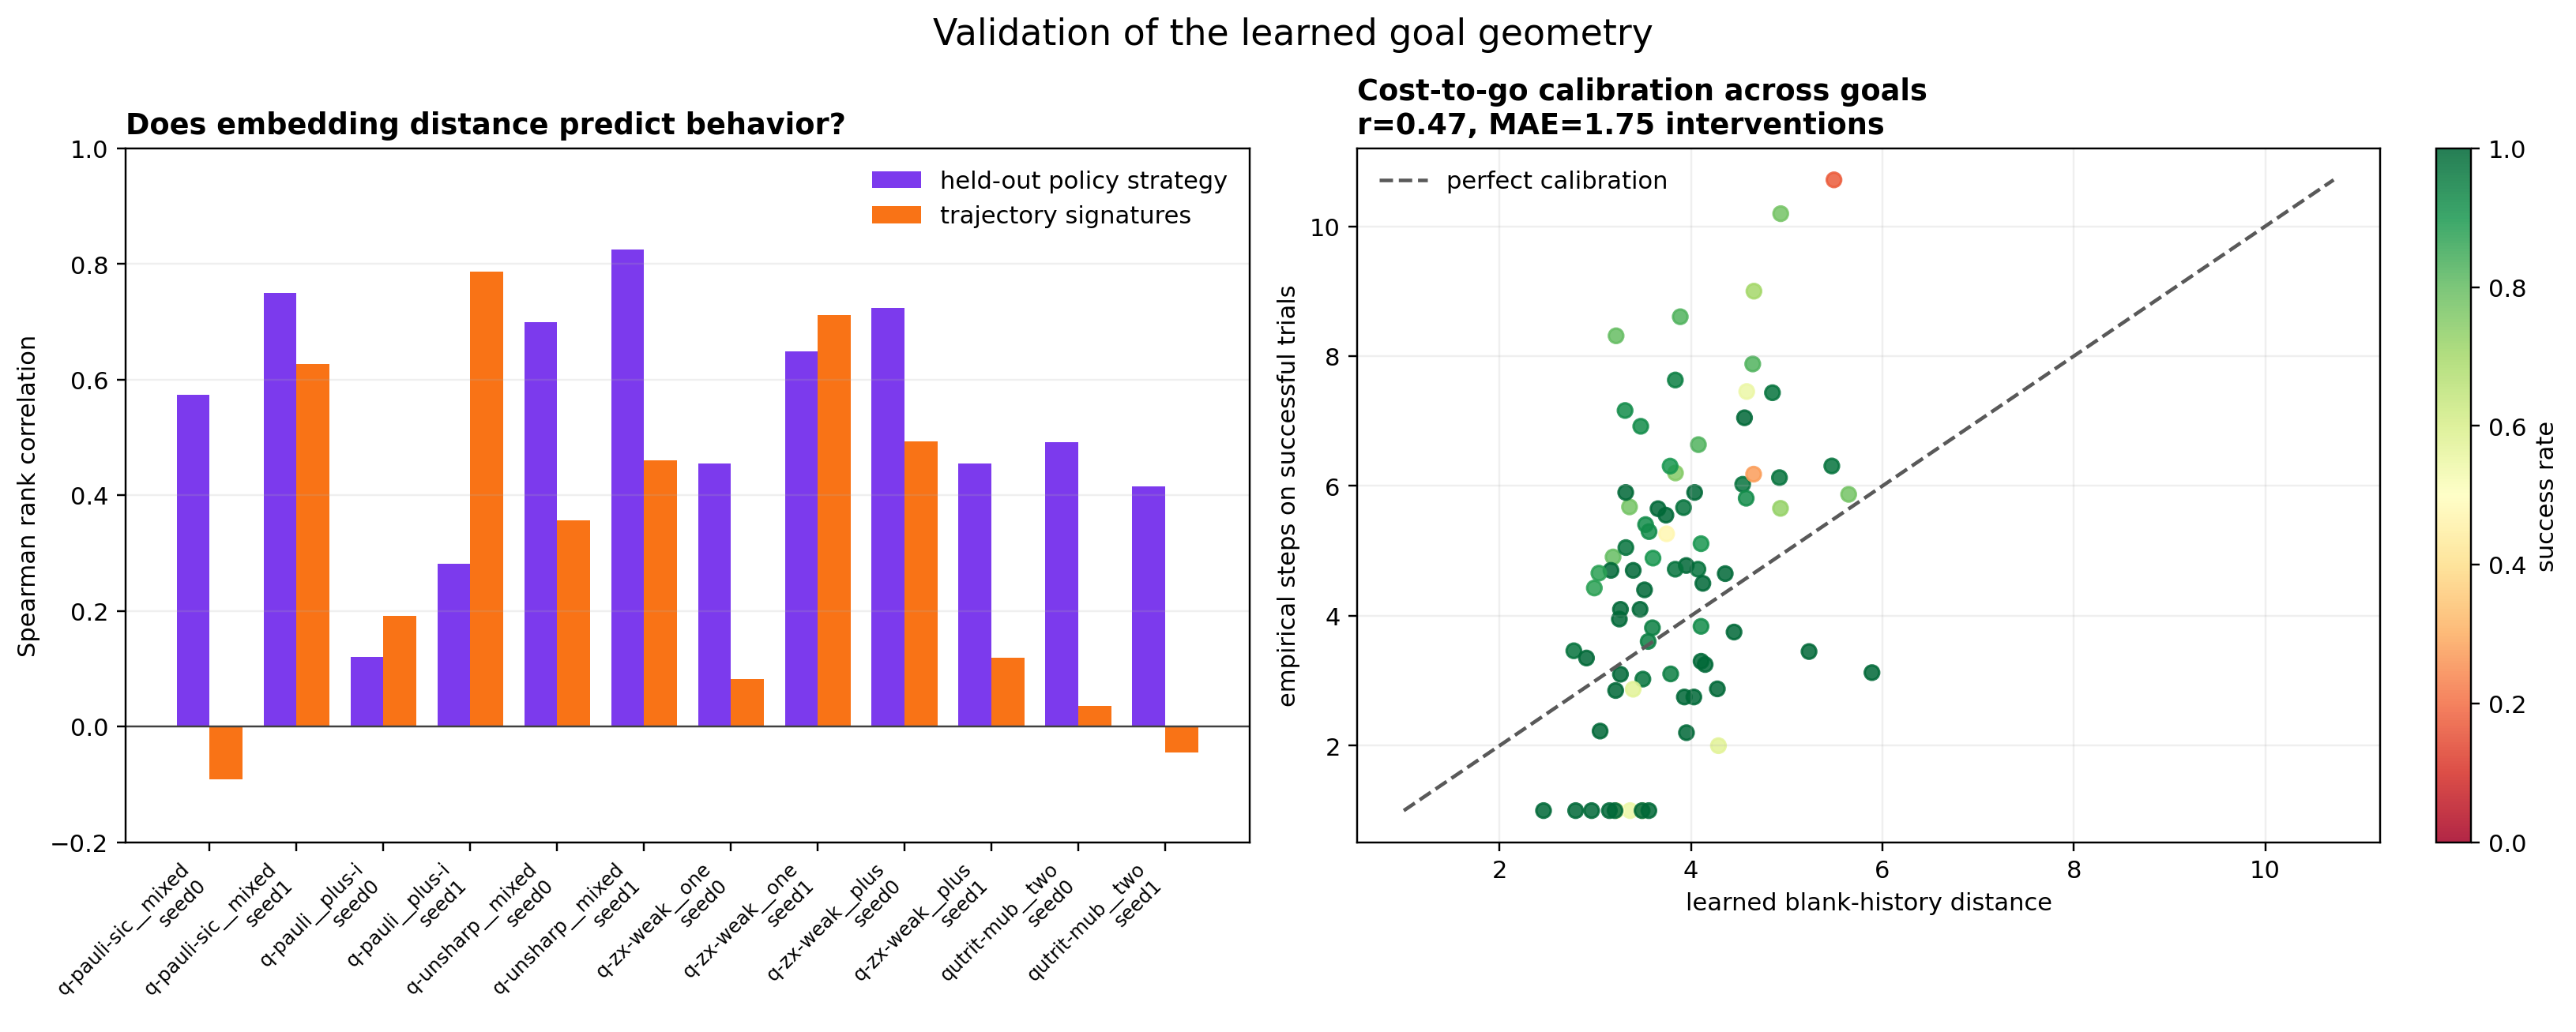
\includegraphics[width=\textwidth]{results/comparative/plots/geometry_validation.png}
\caption{Left: correlation of embedding distance with held-out policy and
trajectory distances. Right: cost-to-go calibration across successful goals.}
\label{fig:validation}
\end{figure}

Across 12 full-agent runs, embedding distance has mean Spearman correlation
$0.537$ with held-out policy strategy distance (median $0.533$, standard
deviation $0.207$, range $0.121$--$0.825$). This is meaningful but imperfect
generalization of the regularized relation. Correlation with more independent
trajectory distance is weaker: mean $0.311$, median $0.274$, standard deviation
$0.303$, range $-0.091$--$0.786$. Geometry is not yet a unique robust object.
The first two PCA axes explain 77.3\% of embedding variance on average.

\begin{figure}[p]
\centering
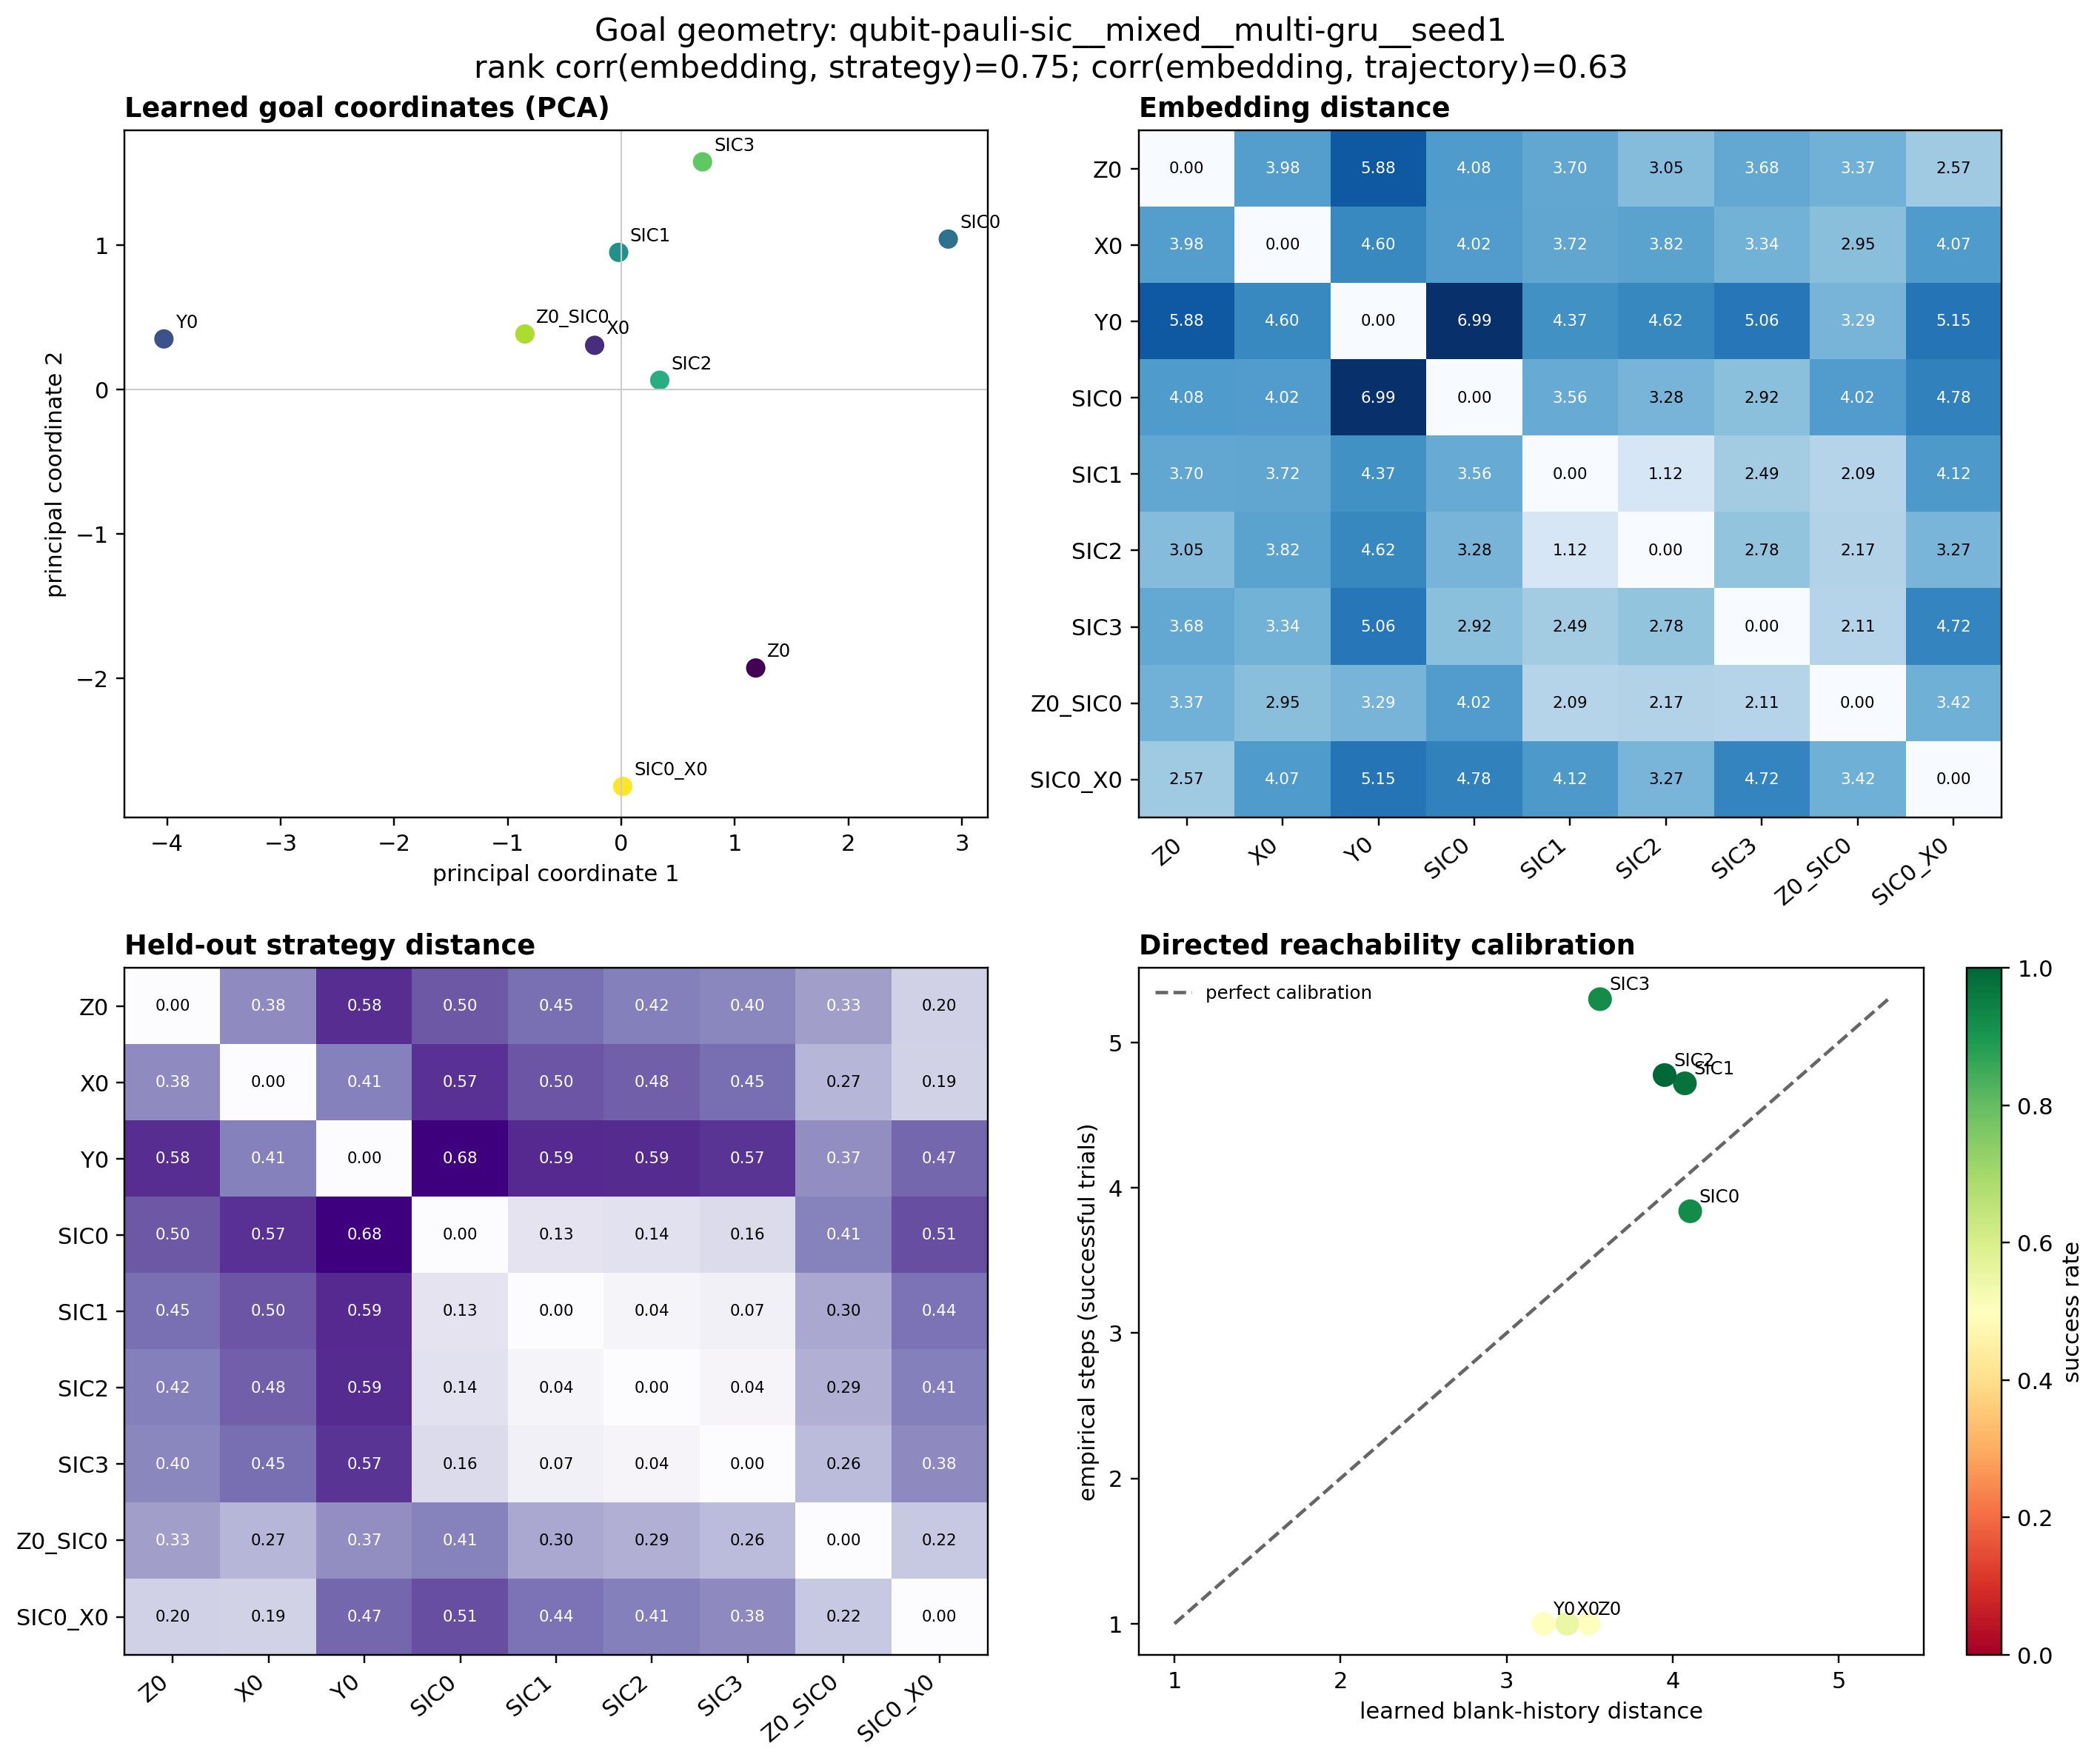
\includegraphics[width=.96\textwidth]{results/comparative/plots/qubit-pauli-sic__mixed__multi-gru__seed1/goal_geometry.png}
\caption{Representative Pauli+SIC geometry (seed 1): PCA coordinates, full
embedding distances, held-out policy distances, and reachability calibration.
The embedding has strategy correlation $0.75$ and trajectory correlation
$0.63$ in this run.}
\label{fig:sicgeo}
\end{figure}

\subsection{Reachability and intervention displacement}

Across 79 goals with at least one geometry-rollout success, predicted cost
correlates $r=0.471$ with conditional empirical steps and has mean absolute
error 1.75. Predictions are compressed to 2.46--5.89 while observed means span
1.0--10.71. The head contains ordinal information but is not a calibrated
clock. Off-policy minimum backups, function approximation, policy mismatch,
finite-horizon censoring, and conditioning on success all contribute.

\begin{figure}[t]
\centering
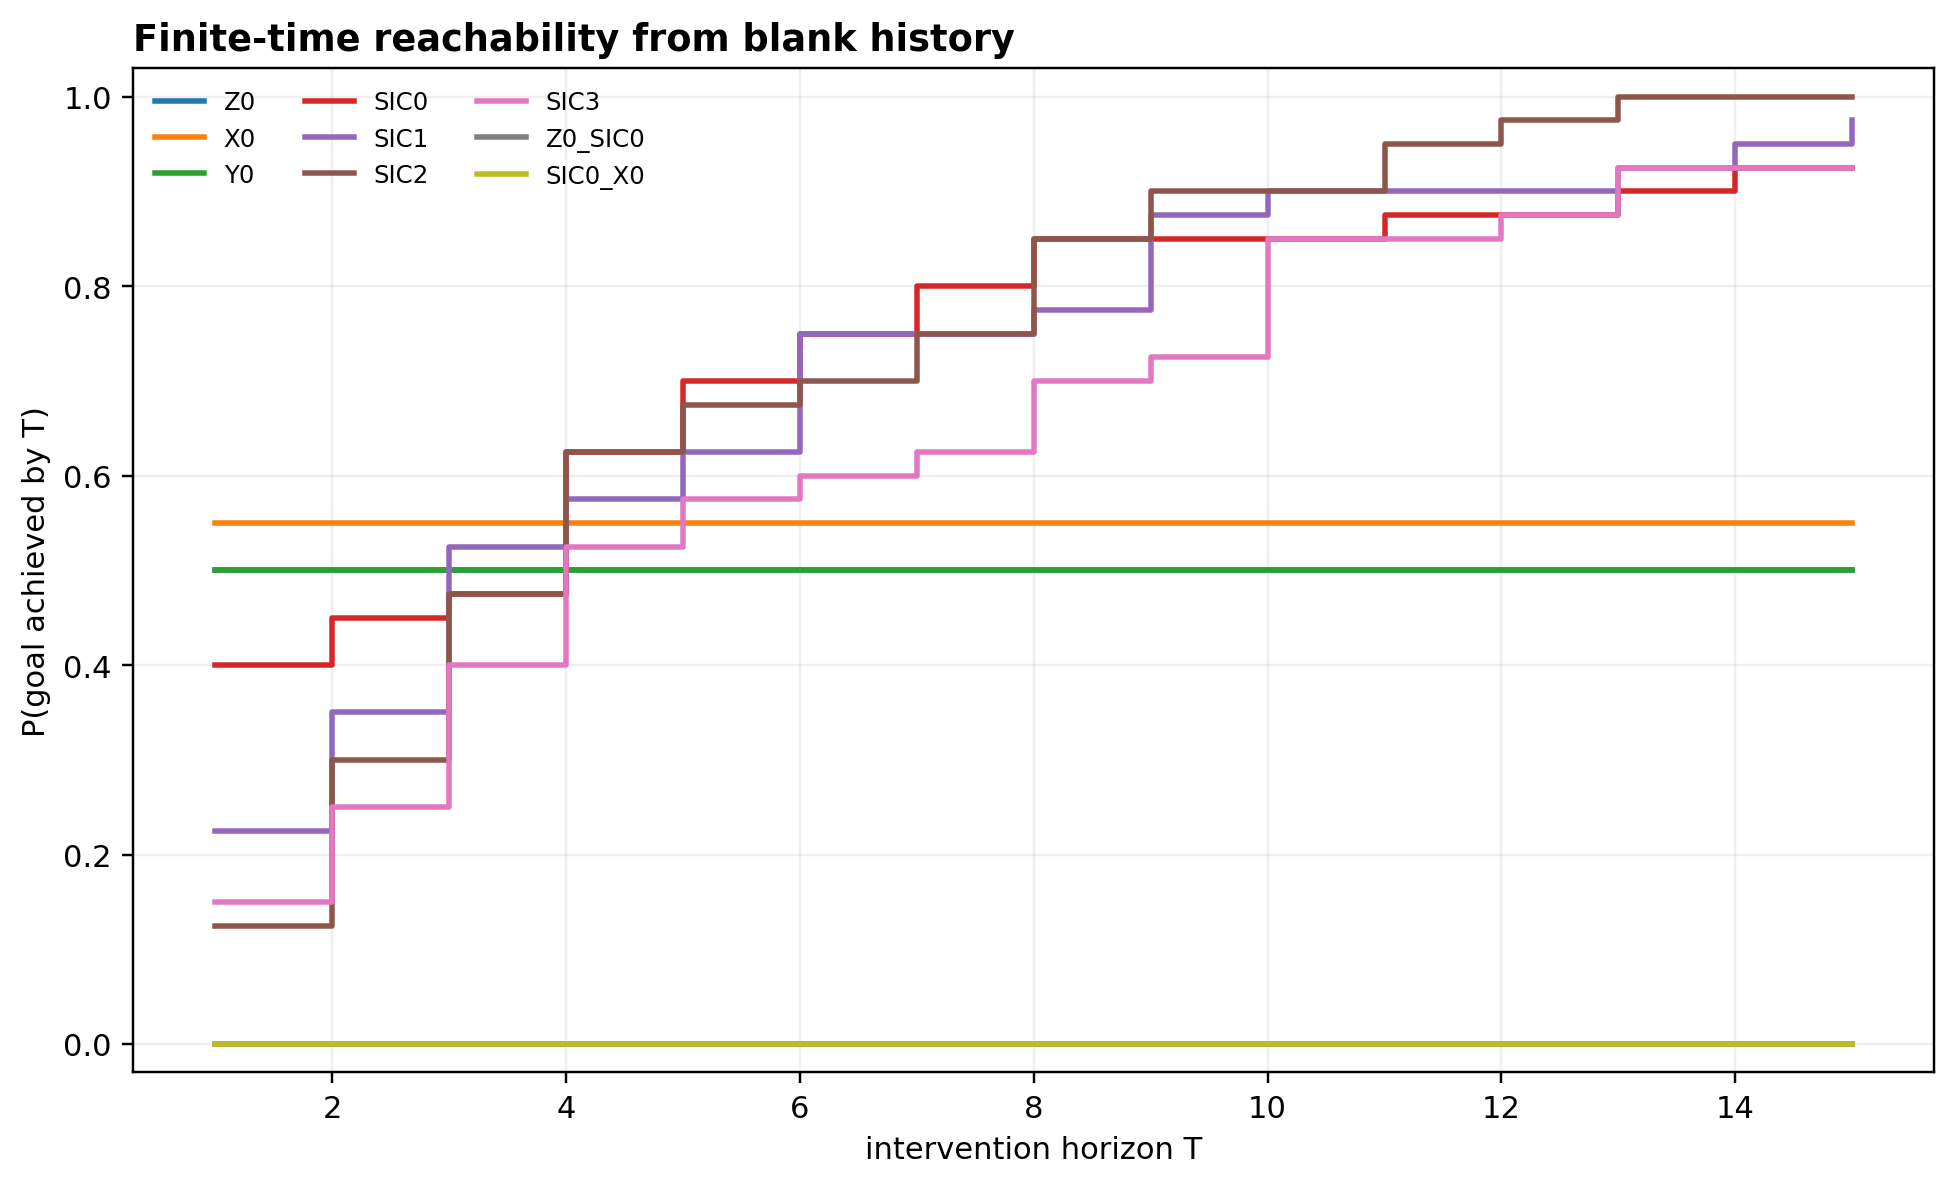
\includegraphics[width=.78\textwidth]{results/comparative/plots/qubit-pauli-sic__mixed__multi-gru__seed1/reachability_curves.png}
\caption{Finite-time success curves retain reliability information hidden by a
conditional mean hitting time.}
\label{fig:curves}
\end{figure}

\begin{figure}[p]
\centering
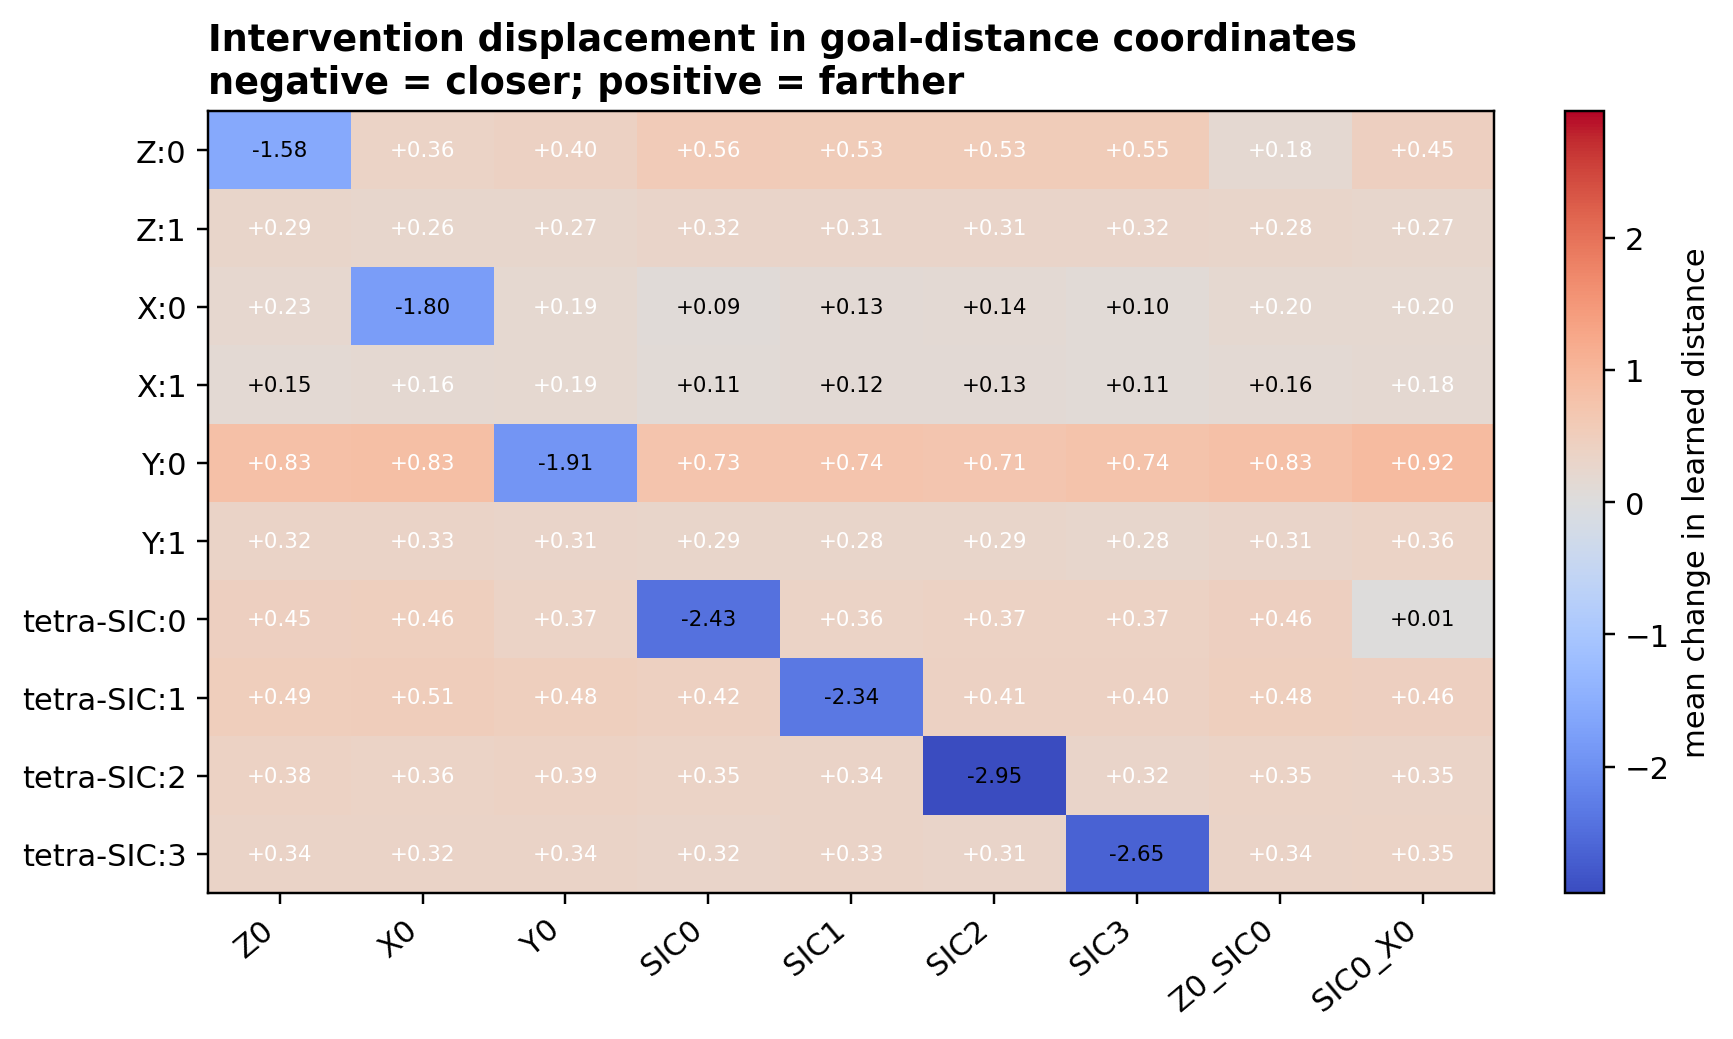
\includegraphics[width=\textwidth]{results/comparative/plots/qubit-pauli-sic__mixed__multi-gru__seed1/intervention_displacements.png}
\caption{Mean displacement in learned goal-distance coordinates. Blue means
closer and red farther. Matching outcomes create strong negative diagonals,
while backaction alters multiple alternative affordances.}
\label{fig:displace}
\end{figure}

In \cref{fig:displace}, $Z{:}0$, $X{:}0$, and $Y{:}0$ change matching-goal
distance by $-1.58$, $-1.80$, and $-1.91$. The four SIC outcomes change their
matching distances by $-2.43$ to $-2.95$, while most nonmatching coordinates
increase. Completion explicitly sets a matching goal to zero, so diagonals
should not be overinterpreted; structured off-diagonal change is the more
interesting signature of backaction.

\section{Discussion and limitations}
\label{sec:discussion}

Useful measurement strategies can be learned without exposing hidden quantum
variables. Recurrent memory sometimes helps, but a short literal history is a
strong small-world baseline. Goal embeddings carry moderate behavioral
meaning, although local policy geometry transfers more reliably than
whole-trajectory geometry. Directed coordinates expose coherent measurement
displacements even though scalar cost is poorly calibrated.

These results do not show that a Bloch sphere, Hilbert space, or uniquely
quantum geometry spontaneously emerged. Such a claim would require latent-state
analysis, intervention ablations, classical controls, and privileged offline
decoding of quantum invariants. Other limitations are:
\begin{itemize}
 \item two seeds cannot support significance claims; modern RL methodology
 recommends more runs, intervals, robust aggregates, and performance profiles
 \cite{agarwal2021};
 \item episode budgets are equal, not compute budgets, and hyperparameters are
 not independently optimized;
 \item horizon 15 censors hard goals, reward shaping affects behavior, and
 conditional steps omit failures;
 \item one-step prediction does not guarantee predictive sufficiency;
 \item goal embeddings are lookup entries and cannot represent unseen goals;
 \item embedding targets come from the same Q-head, creating shared-error and
 circularity risks despite held-out evaluation;
 \item cost is learned off-policy from reward-oriented behavior and is not
 constrained to satisfy stochastic-shortest-path consistency;
 \item simulators omit Hamiltonian dynamics, decoherence, detector error,
 latency, and hardware drift.
\end{itemize}

\section{Outlook}
\label{sec:outlook}

\paragraph{Compositional goals and transfer.}
Encode checkpoint sequences with a GRU or transformer, hold out complete goals,
and test zero/few-shot transfer. Geometry matters if proximity predicts
adaptation speed. Successor features provide a principled comparison
\cite{barreto2017}.

\paragraph{Multi-step predictive state.}
Train action-conditional predictions over entire future tests, compare
recurrent and transformer memory, and measure predictive calibration by
horizon. Vary informational completeness to determine which latent dimensions
disappear.

\paragraph{Planning in possibility space.}
Use \cref{eq:planning} to compare direct Q-control, greedy distance reduction,
and tree search through imagined outcomes. The learned geometry should improve
decisions, not only visualization.

\paragraph{Distributional reachability.}
Learn $\tau_g$ distributions or $R_g(z,T)$ directly, using proper scoring rules
and reliability plots. Distributional Bellman methods are a starting point
\cite{bellemare2017}.

\paragraph{Directed non-Euclidean structure.}
Explore directed graphs, asymmetric energy models, quasimetrics, hyperbolic
goal hierarchies, and Finsler-like local costs. Choose geometry through
predictive validity and planning utility, not aesthetics.

\paragraph{Information-seeking action.}
Replace undirected epsilon exploration with expected information gain,
prediction uncertainty reduction, or reachability uncertainty reduction. This
turns experimentation itself into goal-directed behavior.

\paragraph{Privileged offline physics.}
Pair learned $z_t$ with hidden Bloch coordinates only after training. Test
decodability, intrinsic dimension, convexity, and equivalence classes; compare
against classical partially observed environments.

\paragraph{Stronger statistics and hardware.}
Use 10--20 seeds, longer budgets, bootstrap intervals, interquartile means, and
performance profiles \cite{henderson2018,agarwal2021}. Then add decoherence,
readout error, continuous weak measurement, and device drift, ultimately
learning from laboratory records as envisioned in model-free quantum control
\cite{sivak2022}.

\section{Conclusion}

An agent beginning only with interventions and outcomes can learn more than a
policy. It can compress history, predict contemplated measurements, compare
aims by behavior, estimate goal-relative reachability, and represent
measurement backaction as movement through future possibility. The present
study makes that program concrete but also establishes a demanding standard:
an attractive embedding is not self-validating. It must predict independent
behavior, transfer, and reachability.

The geometry-aware agent is competitive but not universally superior. Its
embedding has measurable, seed-dependent strategic meaning; its directed cost
orders some goals but is not accurate in absolute units. These shortcomings
identify the next experiments. The long-term prospect is an agent not handed a
physical state space, but able to construct a predictive present and a geometry
of possible aims from action and consequence alone.

\appendix
\section{Reproduction and artifacts}

\begin{verbatim}
conda run -n qbist_spacetime python run_experiment_suite.py \
  --scenarios qubit-zx-weak:one,qubit-zx-weak:plus,\
qubit-pauli:plus-i,qubit-unsharp:mixed,\
qubit-pauli-sic:mixed,qutrit-mub:two \
  --backends tabular,gru,multi-gru --seeds 0,1 \
  --episodes 400 --eval-episodes 100 --geometry-episodes 40 \
  --max-steps 15 --epsilon-decay 0.99 --device cpu \
  --output results/comparative
python plot_results.py results/comparative
\end{verbatim}

The manifest records exact runs; episode CSVs retain raw outcomes; geometry
directories store embeddings, three distance views, reachability, curves, and
displacements; and the plot tree contains 51 figures.

\section{Goal repertoires}

\begin{description}[style=nextline]
\item[qubit-zx-weak] $Z0,Z1,X0,X1,Z0\_X0,X0\_Z0,weakZ0\_Z0$.
\item[qubit-pauli] $Z0,X0,Y0,Z0\_X0,X0\_Z0,Y0\_X1,Z0\_X0\_Y0$.
\item[qubit-unsharp] $wZ0,wX0,wY0,wZ0\_wX0,wX0\_wZ0,wZ0\_wX0\_wY0$.
\item[qubit-pauli-sic] $Z0,X0,Y0,SIC0,SIC1,SIC2,SIC3,Z0\_SIC0,SIC0\_X0$.
\item[qutrit-mub] $Z0,Z1,Z2,F0,F1,Z0\_F0,F0\_Z0,Z0\_F0\_P0$.
\end{description}

\begin{thebibliography}{99}
\bibitem{fuchs2014} C.~A. Fuchs, N.~D. Mermin, and R.~Schack,
“An introduction to QBism with an application to the locality of quantum
mechanics,” \emph{American Journal of Physics} 82, 749--754 (2014).
\doi{10.1119/1.4874855}.
\bibitem{kraus1983} K.~Kraus, \emph{States, Effects, and Operations}
(Springer, 1983). \doi{10.1007/3-540-12732-1}.
\bibitem{nielsen2010} M.~A. Nielsen and I.~L. Chuang,
\emph{Quantum Computation and Quantum Information}, 10th anniversary ed.
(Cambridge University Press, 2010). \doi{10.1017/CBO9780511976667}.
\bibitem{renes2004} J.~M. Renes, R.~Blume-Kohout, A.~J. Scott, and C.~M. Caves,
“Symmetric informationally complete quantum measurements,”
\emph{Journal of Mathematical Physics} 45, 2171--2180 (2004).
\doi{10.1063/1.1737053}.
\bibitem{durt2010} T.~Durt, B.-G. Englert, I.~Bengtsson, and K.~\.{Z}yczkowski,
“On mutually unbiased bases,” \emph{International Journal of Quantum
Information} 8, 535--640 (2010). \doi{10.1142/S0219749910006502}.
\bibitem{sutton2018} R.~S. Sutton and A.~G. Barto,
\emph{Reinforcement Learning: An Introduction}, 2nd ed. (MIT Press, 2018).
\url{https://mitpress.mit.edu/9780262039246/reinforcement-learning/}.
\bibitem{watkins1992} C.~J. C.~H. Watkins and P.~Dayan, “Q-learning,”
\emph{Machine Learning} 8, 279--292 (1992). \doi{10.1007/BF00992698}.
\bibitem{kaelbling1998} L.~P. Kaelbling, M.~L. Littman, and A.~R. Cassandra,
“Planning and acting in partially observable stochastic domains,”
\emph{Artificial Intelligence} 101, 99--134 (1998).
\doi{10.1016/S0004-3702(98)00023-X}.
\bibitem{littman2001} M.~L. Littman, R.~S. Sutton, and S.~Singh,
“Predictive representations of state,” in \emph{NeurIPS 14} (2001).
\url{https://papers.nips.cc/paper/2001/hash/1e4d36177d71bbb3558e43af9577d70e-Abstract.html}.
\bibitem{cho2014} K.~Cho et al., “Learning phrase representations using RNN
encoder--decoder,” in \emph{EMNLP}, 1724--1734 (2014).
\doi{10.3115/v1/D14-1179}.
\bibitem{mnih2015} V.~Mnih et al., “Human-level control through deep
reinforcement learning,” \emph{Nature} 518, 529--533 (2015).
\doi{10.1038/nature14236}.
\bibitem{bertsekas1991} D.~P. Bertsekas and J.~N. Tsitsiklis,
“An analysis of stochastic shortest path problems,”
\emph{Mathematics of Operations Research} 16, 580--595 (1991).
\doi{10.1287/moor.16.3.580}.
\bibitem{endres2003} D.~M. Endres and J.~E. Schindelin,
“A new metric for probability distributions,”
\emph{IEEE Transactions on Information Theory} 49, 1858--1860 (2003).
\doi{10.1109/TIT.2003.813506}.
\bibitem{barreto2017} A.~Barreto et al., “Successor features for transfer in
reinforcement learning,” in \emph{NeurIPS 30} (2017).
\url{https://papers.nips.cc/paper/6994-successor-features-for-transfer-in-reinforcement-learning}.
\bibitem{bellemare2017} M.~G. Bellemare, W.~Dabney, and R.~Munos,
“A distributional perspective on reinforcement learning,”
\emph{Proceedings of Machine Learning Research} 70, 449--458 (2017).
\url{https://proceedings.mlr.press/v70/bellemare17a.html}.
\bibitem{henderson2018} P.~Henderson et al., “Deep reinforcement learning that
matters,” in \emph{AAAI} (2018). \doi{10.1609/aaai.v32i1.11694}.
\bibitem{agarwal2021} R.~Agarwal et al., “Deep reinforcement learning at the
edge of the statistical precipice,” in \emph{NeurIPS 34}, 29304--29320 (2021).
\url{https://papers.nips.cc/paper/2021/hash/f514cec81cb148559cf475e7426eed5e-Abstract.html}.
\bibitem{fosel2018} T.~F\"osel, P.~Tighineanu, T.~Weiss, and F.~Marquardt,
“Reinforcement learning with neural networks for quantum feedback,”
\emph{Physical Review X} 8, 031084 (2018).
\doi{10.1103/PhysRevX.8.031084}.
\bibitem{sivak2022} V.~V. Sivak et al., “Model-free quantum control with
reinforcement learning,” \emph{Physical Review X} 12, 011059 (2022).
\doi{10.1103/PhysRevX.12.011059}.
\bibitem{borah2021} S.~Borah et al., “Measurement-based feedback quantum
control with deep reinforcement learning for a double-well nonlinear
potential,” \emph{Physical Review Letters} 127, 190403 (2021).
\doi{10.1103/PhysRevLett.127.190403}.
\end{thebibliography}

\end{document}
